\chapter{Theoretical introduction}
\label{sec:Theory}

In this section the theoretical basis for the measures will be explained. First of all, the overview of the standard model, then the theoretical aspects of the $pp$ collisions, and in the end the specifies of the $Z$ boson production.

\section{The Standard Model}
\label{sec:theory_SM}

The standard model is a theoretical foundation of all of modern particle physics. It described all of the currently-known particles and three out of four currently-known types of interactions (being weak, strong, and electromagnetic, excluding gravity). It was developed during the last fifty years and made several predictions on the nature of particles and interactions, all which were confirmed by the present time. Among its predictions were quarks (first confirmed in mid 1970s), vector bosons (confirmed in 1983), top-quark (confirmed in 1995), and $\tau$-neutrino (confirmed in 2000). The last to-date update to the standard model was made in 2002 with the theoretical explanation of neutrino oscillations, which was confirmed to be true with the T2K experiment in july 2013. The most recently confirmed major prediction of the standard model was the existence of the Higgs boson, which was confirmed in january 2013.

The main theses of the standard model are:
\begin{itemize}
\item There are 61 fundamental particles which can be divided into several groups (can be seen on Fig.~\ref{fig:THEORY_SM}):
\begin{itemize}
\item The quarks, which have electromagnetic weak and color charge, and thus participate in all three interactions. There are two types of quarks defined by their charges, three generations for each, and 3 possible color charges. Together with the anti-particle partner for every particle this makes 36 particles in total.
\item The leptons, which do not have color charge, and thus do not participate in strong interactions. Again, there are two types of leptons, one having both electric and weak charges and one having only the weak, three generations for each and possible anti-particle partner, which makes the total of 12.
\item The gauge bosons, the force carriers for all three fundamental interactions, which can be divided into three symmetry groups: the gluons, carriers of the strong interaction with 8 possible color charges, constituting the $SU(3)$ group; the $W^{\pm}$ and $Z$ bosons, carriers of the weak interaction, constituting the $SU(2)$ group; the photons, carriers of the electromagnetic interaction, constituting the $U(1)$ group. The total number of gauge bosons is thus 12.
\item The Higgs boson, by interacting with which all other particles gain their masses.
\end{itemize}
\item The quarks and leptons, together known as fermions, are participating in the interactions. The strong and electromagnetic interactions only occur between the fermions in the same generation, while the weak interaction can mix the generations, which enables fermions to weakly decay into lighter particles.
\item The standard model has several parameters which can not be theoretically predicted: the masses of all massive particles, the gauge couplings, the CKM mixing angles and the Weinberg angle (Tab.~\ref{tab:SM_parameters}).
\end{itemize}

\begin{figure}
\center{
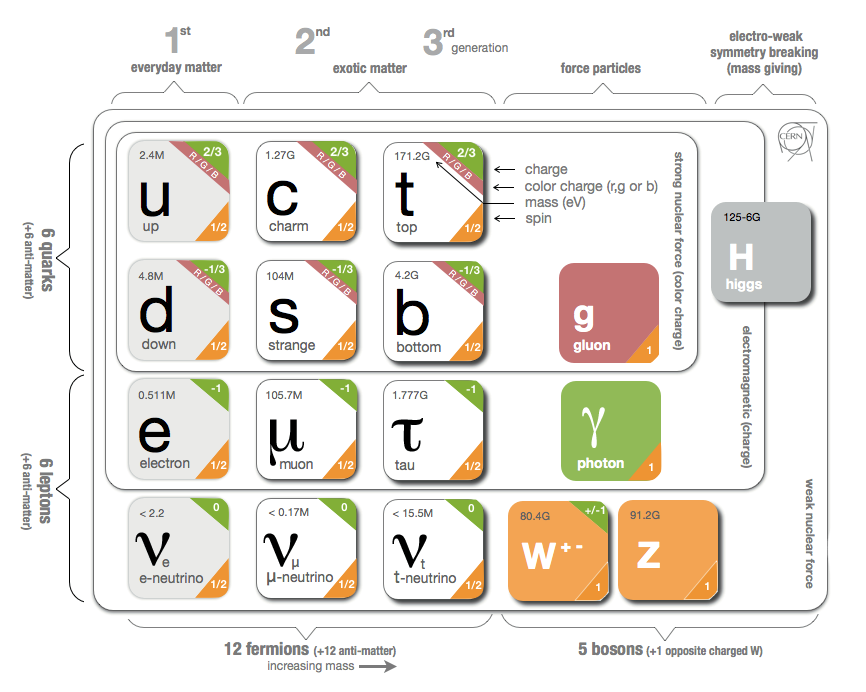
\includegraphics[width=0.95\textwidth]{figures/THEORY_SM.png}
\caption{The particles of the standard model. The image was made during 2012 CERN Summer Student Webfest.}
\label{fig:THEORY_SM}}
\end{figure}

\begin{table}[ht!]
\centering
\begin{tabular}{c|c|c} \hline\hline
Parameter & Description & Value \\\hline

$m_{u}$ & Up quark mass &  1.9 MeV \\
$m_{d}$ & Down quark mass & 4.4 MeV \\
$m_{s}$ & Strange quark mass & 87 MeV \\
$m_{c}$ & Charm quark mass & 1.32 GeV \\
$m_{b}$ & Bottom quark mass & 4.24 GeV \\
$m_{t}$ & Top quark mass & 172.7 GeV \\
\hline
$m_{e}$ & Electron mass & 511 keV \\
$m_{\mu}$ & Muon mass & 105.7 MeV \\
$m_{\tau}$ & Tau mass & 1.78 GeV \\
\hline
$m_{Z}$ & Z boson mass & 91.18 GeV \\
$m_{W}$ & W boson mass & 80.38 GeV \\
$m_{H}$ & Higgs boson mass & 126 GeV \\
\hline
$\alpha$ & Fine-structure constant & $7.297 \cdot 10^{-3}$\\
$\alpha_{s}(m_Z)$ & Strong coupling constant & 0.1184\\
$G_{F}/(\hbar c)^3$ & Weak coupling constant & $1.166 \cdot 10^{-5}$ \\
\hline
$sin^{2} \Theta_{W}$ & Weinberg angle & 0.231 \\
%\hline
%$\Theta_{12}$ &\multirow{3}{*}{CKM mixing angles}& $13.1^{\circ}$ \\
%$\Theta_{13}$ && $0.2^{\circ}$ \\
%$\Theta_{23}$ && $2.4^{\circ}$ \\
%$\delta_{13}$ & CKM CP-violating Phase & 0.995 \\
\hline\hline
\end{tabular}
\\[2ex]
$V_{CKM} = \left(\begin{array}{ccc}
0.9742 & 0.2253 & 0.0035 \\
0.2252 & 0.9734 & 0.0412 \\
0.0086 & 0.0404 & 0.9991 \\
\end{array}\right)$
\caption{The list of the parameters of the standard model, assuming the masses of neutrinos are zeros.}
\label{tab:SM_parameters}
\end{table}

The standard model is not a single theory which describes everything, it's a system of several interconnected theories which were developed in different times, sometimes replacing one another as new experimental data was found. At the start of the 20th century the dominant idea in physics was that of the electromagnetic aether~\cite{lib:theory_EM1, lib:theory_EM2, lib:theory_EM3}. The aether was believed to be the source of all matter, as well as both the EM and gravitational forces. When the electron was discovered in 1897~\cite{lib:theory_electron} it was regarded as tool for the further development of the aether theory as the "theory of everything", because the observable properties of the electron suggested that it had no "not-electromagnetic" features (i.e. no mass). The high peak of the aether theory was in 1904 when Walter Kaufmann discovered the velocity dependence of the $e/m$ ratio in cathode rays~\cite{lib:theory_e_m1, lib:theory_e_m2}, which fell in line with the concept of the electromagnetic impulse previously suggested by Henri Poincare and Max Abraham. At the same time, the new concept of the relativity was developed by Hendrik Lorentz and Albert Einstein~\cite{lib:theory_relat}. The theory also marked the beginning of the completely new approach (which can be called a "relativistic program" as opposed to the previously established "aetherial field program") to the theoretical physics which was one of the reasons why physicist were so reluctant to accept it. It was only in 1911, after the works of Hermann Minkowski~\cite{lib:theory_minkowski1, lib:theory_minkowski2}, when the concept of the relativity became widely accepted.

But even after the acceptance of the idea of relativity, there were some efforts to keep the aether model as the basis for all matter. The most notable theories were made by Gustav Mie. His mathematical models that were made in 1912-1913 were supposed to describe both particles (e.g. electrons) and EM interaction (which was believed to be universal and include gravity as well), and they should also be able to mathematically predict fundamental constants, such as electron charge and $\hbar$, also known as Planck's constant, and is a fundamental constant that links the energy of the quantum with it's frequency. Mie believed that the quantum effects could be described electromagnetically, because the Planck's constant $\hbar$ was found to be the same order of magnitude as $e^{2}/c$ (which was previously noted by Einstein, who also tried to construct the similar mathematical theory 1908 with no results). But the theory was never finished, the lagrangian for it was never found, even though several physicists tried to find it even in 1930s-1940s, long after the establishment of the quantum theories. These works also inspired several other attempts to build a unified field theory, such as Jun Ishihara and Gunnar Nordstr{\"o}m in 1914, David Hilbert in 1915, Hermann Weyl in 1919, and finally, the Kaluza-Klein theory in 1921 which was the first theory to introduce the extra dimension, and thus became the foundation of the string theory.

But in the 20s, all the approaches to construct a field theory that would describe the EM interaction and also have a non-singular, spherically-symmetrical, statical solutions that can be interpreted as electrons failed. And it was during that time when quantum physics made the biggest progress. The theory was quickly established by predicting different spectroscopy results. The biggest milestones were the hypothesis of Louis de Broglie, who postulated the wave-particle duality in 1924, the development of the matrix mechanics by Werner Heisenberg, Max Born, and Pascual Jordan in 1925, and finally the establishment of the equivalence of wave and matrix approaches in 1926. The non-deterministic nature of the quantum mechanics was formulated by Heisenberg in 1927. On the fifth Solvay Conference\footnote{A Solvay Conference is a conference established by International Solvay Institutes for Physics and Chemistry in 1911, and is widely regarded a turning point of the modern physics.} that was held that year, the quantum physics was fully established as the new program for the theoretical physics. All this culminated in the Dirac's equation which was introduced in 1928, and unified the quantum physics with the theory of relativity.

\begin{equation}
(i \hbar c \gamma^{\mu} \dd_{\mu} - m c^{2})\Psi = 0\,.
\end{equation}

It allowed to theoretically calculate the energy levels of the hydrogen including the fine structure, and explain Zeeman's effect. Based on this equation the formulaes for the Compton scattering were calculated as well as for the bremsstrahlung, which was later observed experimentally. It also predicted the existence of the anti-matter, as a physical interpretation of the solutions with the negative energy (the positrons were first discovered in 1932). It could be used to described all the half-integer spined non-interacting particles. The following efforts to include the EM interaction in it resulted in the quantum electrodynamics theory.

\subsection{Quantum Electrodynamics (QED)}

The main effort in fundamental physics since the discovery of the particles was the unification of the particles and interactions in a single theory. The class of theories that was searched for it was the geometrical field theories, and the most notable figures in that search were Einstein and Weyl. The geometrical field approach never gave any successful theories, but it laid the foundation for the pivotal point of the modern standard model: the gauge field theory.

It was Weyl's theory that he developed in the 1919 that was put as the basis of the first gauge theory, that he developed together with Vladimir Fock and Fritz London. Fock was the one to introduce the first version of the local gauge transformation:

\begin{equation}
\begin{split}
\psi^{'} &= e^{-i\frac{ef(x)}{hc}}\psi \,,\\
\varphi^{'}_{i} &= \varphi_{i} + \frac{\dd f(x)}{\dd x_{i}} \,.
\end{split}
\end{equation}

The gauge theory is a type of a field theory which has the so-called gauge invariance or gauge symmetry - the property in which different configurations of the underlying fields, which are not themselves directly observable, result in identical observable quantities. The example of the simple transformation which will satisfy this criteria can be constructed using the local $U(1)$ symmetry group:

\begin{equation}
\Psi(x) \to e^{i\alpha(x)}\Psi(x)\,.
\end{equation}

The term $e^{i\alpha(x)}$ is complex and thus can't be observed, but we also need the equation describing the particle to be invariant to this transformation, and with this restriction the equation describing the interacting particles can be derived:

\begin{equation}
\begin{gathered}
L = \bar \Psi (i \gamma_{\mu} \dd^{\mu} - m) \Psi + e \bar \Psi \gamma_{\mu} A^{\mu} \Psi - \frac{1}{4} F_{\mu\nu}F^{\mu\nu}\\
F_{\mu\nu} = \dd_{\mu}A_{\nu} - \dd_{\nu}A_{\mu}\,.
\end{gathered}
\end{equation}

The vector field $A_{\mu}$ introduced in this equation is the electromagnetic field and it allows us to achieve the desired invariance. The term $e \bar \Psi \gamma_{\mu} A_{\mu} \Psi$ describes the interaction between this field and the particle, and the term $F_{\mu\nu}F^{\mu\nu}$ represents the kinetic energy of the field itself and is in accordance with the Maxwell's equations for the electromagnetic interactions.

The development of the gauge theory continued with the works of Fermi, Dirac, Fock, Heisenberg and was finally formulated in 1954 in the work of Chen Ning Yang and Robert Mills. At first, the Yang-Mills theory found no application in quantum field theories, and it had some internal problems, like the unability of quantization for non-abelian groups (e.g. $SU(2)$, which by that time was already proposed for the weak interaction). The quantization of the Yang-Mills fields for non-abelian groups was done later with the help of the previous works of Ludvig Faddeev and Victor Popov who introduced the so-called Faddeev-Popov ghosts.

The inclusion of the weak interaction first was attempted by Enrico Fermi in 1933. His theory didn't involve any interaction carriers, with particles interacting directly in one vertex. And while it described the results of the $\beta$-decay remarkably well, the need for a more elaborate description of different occurrences of the new type of interaction became gradually stronger as new experimental data was collected. The most notable was the "Wu experiment" conducted in 1956 by Chien-Shiung Wu which established the violation of the P-symmetry\footnote{The "P-symmetry", or "parity symmetry" is the idea that the quantum processes would remain the same if we swap "left" and "right". The processes that make difference between "left" and "right" are said to "violate the P-symmetry".}. The next attempt to develop a theory was done a year later after that in 1957 by Robert Marshak and George Sudarshan and also independently by Richard Feynman and Murray Gell-Mann. The theory they developed was called a $V-A$ theory as "vector minus axial vector" after the main term of the Lagrangian that described the interaction. In 1964 the CP violation\footnote{Much like the P-symmetry, the CP-symmetry is the idea that the processes would remain the same if we change both the parity and the charges, i.e. change the matter into antimatter and vise versa. The CP-symmetry was introduced after the confirmation of the P-symmetry violation as the new fundamental symmetry of the quantum processes.} was observed in the kaon experiment by James Cronin and Val Fitch. The $V-A$ theory couldn't explain it, so there was a need to either update the $V-A$ theory or to introduce the new theory of some "superweak interaction". And at first, such superweak theories were developed, so when the new theory (that later became the QED theory) was developed by Sheldon Glashow, Steven Weinberg, and Abdus Salam in 1968, that was based on the gauge Yang-Mills theory, it wasn't accepted. By that time the theory had several internal problems, but most importantly, it also wasn't able to describe the CP-violation. The first important advantage of the new theory was gained in 1972, when Gerard 't Hooft and Martinus Veltman proved that the Yang-Mills fields were renormalizable\footnote{The renormalization of the theory is important for the use of the perturbation theory to predict the outcomes of the interactions. If the theory is not remormalizable, the integrals produced by the perturbation theory will divergent.}. They shared a Nobel prize for that work in 1999. And it was finally accepted in 1973, when the Gargamelle bubble chamber at CERN presented the direct evidence of the existence of neutral currents, that were predicted by their theory. The new gauge bosons, $W$ and $Z$, were directly observed only in 1983. In the same 1973 the first works appeared that proved that the gauge theory can explain the CP-violation if the third generation of quarks were to be added. This discovery would be further discussed in the following section.

\subsection{Quantum Chromodynamics (QCD)}

The firsts works on the theory of the strong interactions started even before this interaction was first observed, as a theoretical explorations of the possibilities of the $SU(3)$ groups in particle physics. The need for the new theory first arose in 1947 after the discovery of the $K$-mesons in cosmic rays. The first attempts to include the new experimental data to the existing theories were made by suggesting, that the new interaction is the same as the EM interaction in nature, but with massive carriers. Considering that

\begin{equation}
\Delta E \cdot \Delta t = (m_{q}c^{2}) \cdot \Delta t \approx \hbar \,,
\end{equation}

where $m_{q}$ is the mass of the field quantum and $\Delta t$ is its lifetime, and considering that $r = c \cdot \Delta t$ where the radius of the strong interaction was predicted to be $r = 10^{-15}$~m we will get the predicted value for the carrier mass as

\begin{equation}
m_{q}c^{2} \approx \frac{\hbar c}{r} \approx 200 \: \mbox{MeV}\,.
\end{equation}

The theoretical works predicting the massive carrier for the strong nuclear force were done by Hideki Yukava in 1935. In 1947 $\pi^{+}$-meson was observed with the mass of 140~MeV, which initially was thought the carrier of the strong interaction. Although technically it wasn't true, the discovery of $\pi$-mesons played a big role in the foundation of the QCD, and Yukava got a Nobel prize in 1949 for his work. Later, in 1950 the $\Lambda^{0}$-baryons were observed in experiments conducted by V. D. Hopper and S. Biswas. These particles had a much longer lifetime than the theories predicted, and it was proposed that they have some new, unknown charge which was called "strange". The number of new particles observed experimentally grew steadily, and there were no successful attempts to fit them into the $SU(2)$ groups.

In 1961 Yuval Ne'eman and later independetly Murray Gell-Mann in 1962 proposed a new hadron classification model, the so-called "eightfold way". It was based on the $SU(3)$ group, and among other things, predicted the $\Omega$-baryon as part of the baryon decuplet. This baryon was found in 1964 with the mass and properties predicted by the model. Yet, the fundamental elements of the $SU(3)$ group were still not described be the theory. This problem was solved with the introduction of the quark model independently by Murray Gell-Mann and George Zweig in 1964. The quark model still had several flaws though. First of all, the quarks that the theory proposed were never observed experimentally. Second, only the \qqbar\ and $qqq$ states were observed, no $qq$ or $qqqq$. There were no rules that forbade such states. And the main issue was the flaws within the theory itself. For example, according to the theory, the $\Delta^{++}$-baryon consisted of three quarks ($uuu$) with the spin $1/2$, which violated the Pauli principle. To solve this problem, there was introduced another charge, called "color". It was first proposed by Oscar W. Greenberg in 1964 as an independent $SU(3)$ group of color charges. This idea was developed for several years and eventually laid the foundation for the modern QCD theory. Murray Gell-Mann got the Nobel prize in 1969 for his works in this field.

In the same year 1964, several works predicted the existence of the fourth quark as part of the quark-lepton symmetry. But the prediction is usually credited to Sheldon Glashow, John Iliopoulos and Luciano Maiani for their work on flavor-changing neutral currents that was published in 1970. The proposed mechanism (the GIM mechanism, for the first letters in the authors names) required the forth quark to exist.

Also in 1964 the works started on the CP-violation in $K$-meson decays. The important work was done by James Watson Cronin and Val Logsdon Fitch who received the Nobel prize for it in 1980. The works on CP-violation were continued by Makoto Kobayashi and Toshihide Maskawa who based it on the work of Nicola Cabibbo on weak interactions, and added a third generation of quarks. They published their work in 1973.

In the same year David Gross, Frank Anthony Wilczek and Hugh David Politzer published their work on asymptotic freedom in strong interaction, which solved the so-called "Landau-pole" problem, which suggested that the interactions should become infinitely strong at certain scale. This work allowed to predict the results of the deep inelastic scattering by the means of perturbative theory. They shared a Nobel prize in 2004 for that work.

In 1974 the $J/\psi$ meson was first observed independently in SLAC and BNL. This particle had a width of a mass peak much smaller that the theory predicted for a particle of this mass. The only explanation for this was an assumption, that the particle was a bound state of an unknown heavy quark that was called "charm" (or c-quark).

The bound state of the second heavy quark - the $\Upsilon$-meson, was discovered in 1977 in Fermilab. The last predicted quark was searched for for the next twenty years because of its very high mass. Only in 1995 it was jointly confirmed by two detectors (DZero and CDF) on Tevatron collider at Fermilab.

Makoto Kobayashi and Toshihide Maskawa got a Nobel prize in 2008 for their work.

\section{Parton Distribution Function (PDF)}
The processes that we observe during the high-energy collisions suggest that the hadrons are complex particles that consist of several partons. The term "parton" was first proposed Richard Feynman in 1969 as a generic term for every particle that constitutes hadrons, now they are called quarks and gluons. At first, the hadrons were believed to consist of duplets (\qqbar) and triplets ($qqq$) of quarks. But, through the interaction processes, these quarks (also called the valence quarks) can also produce an arbitrary number of the lower-energy virtual partons, also called "sea" quarks and gluons. The sea partons were first observed by James Bjorken and Emmanuel  Paschos in 1969.

Every parton within the hadron carries some amount of it's energy. So in order to predict the results of the deep inelastic scattering involving a hadron we need to calculate which parton will be participating in the scattering and what fraction of the hadron's energy it carries. These parameters can't be derived from the theory in any way, they can only be produced based on the experimental data, which leaded to the creation of the parton distribution functions.

\begin{figure}
\center{
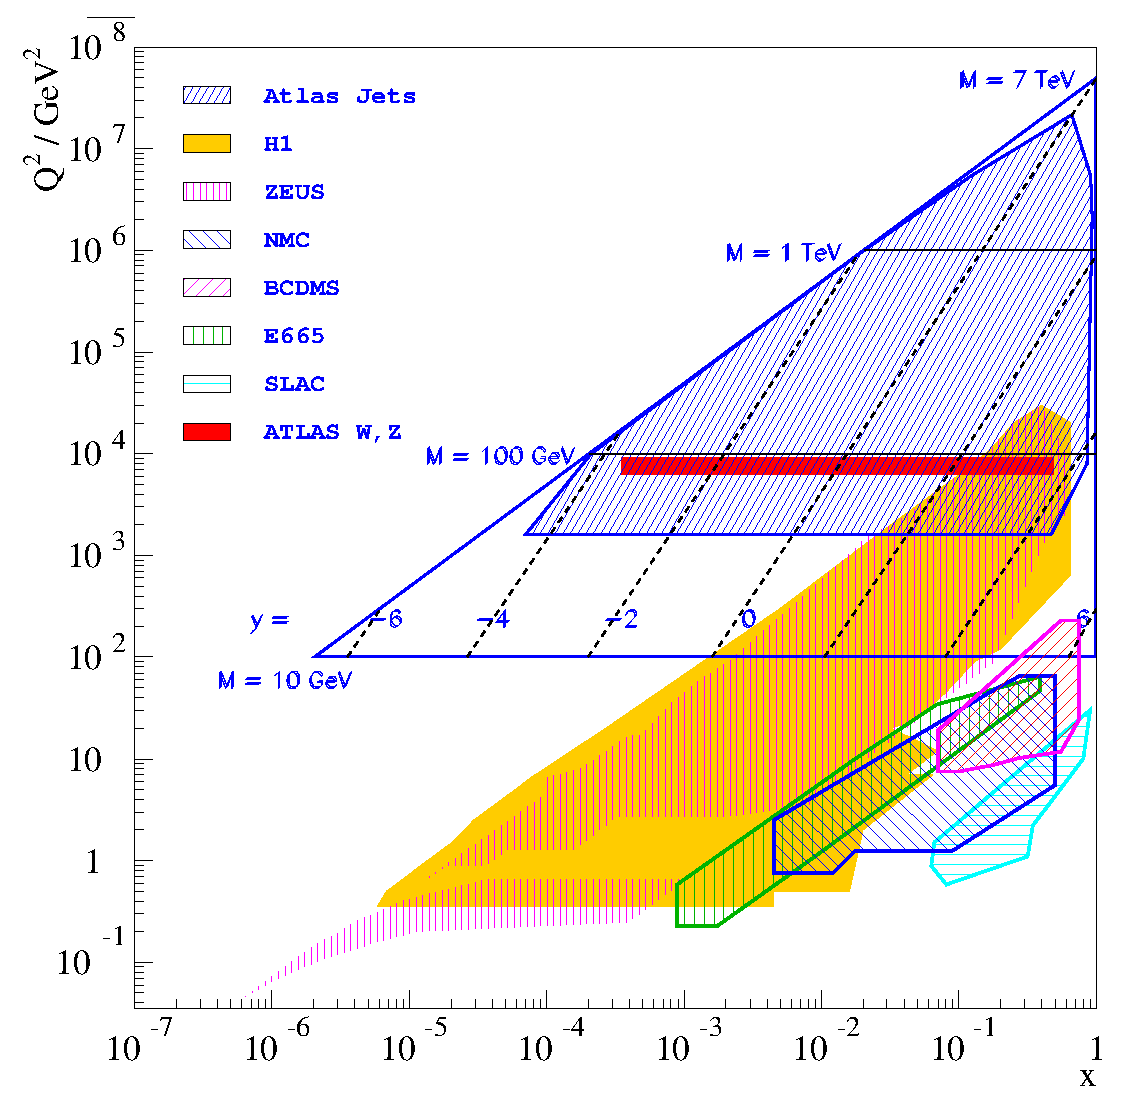
\includegraphics[width=0.65\textwidth]{figures/THEORY_PDF.eps}
\caption{The kinematic plane of various collider experiments in $Q^{2}$ and $x$. In red the range for Z and W production in ATLAS is shown.}
\label{fig:THEORY_PDF}}
\end{figure}

The PDF is a function that shows the probability of finding the given parton in the given hadron with a given momentum. In the collision experiments the most interest represent the proton PDFs which are constructed based on the experimental data from the $ep$, $pp$ and $\antibar{p}$ scattering. The proton PDFs depend on two parameters: "$Q^{2}$" and "Bjorken $x$" (or just "$x$"). The $Q^{2}$ is a measure of the combined energy of the particles that participate in the collision, and $x$ represents the momentum fraction of the proton that the interacting parton holds. The constructed PDFs are only applicable for the certain range of $Q^{2}$ and $x$, which depends on the range coverage of the data they were based on. The coverage of the kinematic plane in $Q^{2}$ and $x$ of various experiments is shown in Fig.~\ref{fig:THEORY_PDF}. The red stripe in the middle is the W and Z boson production in ATLAS. It can be seen that the $Q^{2}$ is very narrow, because these analyses only cover a mass window of $46 < M < 150$~GeV (and even less so in case of central-forward analysis), while the $x$ coverage is quite wide. As it can be seen on the plot, the $x$ parameters is tied with the boson rapidity, which in turn translates to the pseudorapidity of the decay products (i.e. electrons, in case of \Zee). The rapidity $y$ and pseudorapidity $\eta$ are defined by these equations:
\begin{equation}
\begin{gathered}
y = \frac{1}{2} \log \left(\frac{E+p_z}{E-p_z}\right)\,, \\
\eta = - \log (\tan (\frac{\theta}{2}))\,.
\end{gathered}
\end{equation}
The $y$ coverage of the \Zee\ central-central analysis (as well as \Zmm\ and \Wenu) is $|y| < 2.4$, while the coverage of $2.4 < |y| < 3.6$ is achieved solely by \Zee\ central-forward, so it is very important in order to produce a wide coverage of the kinematic plane.

To scale PDFs the evolution equations must be used, such as DGLAP. To accurately predict the results of hadron scattering the set of 13 different PDFs is required, one for each of the 12 quarks ($\bar{t}$, $\bar{b}$, $\bar{c}$, $\bar{s}$, $\bar{u}$, $\bar{d}$, $d$, $u$, $s$, $c$, $b$, $t$) and one for the gluons. The color of the partons can't be determined, so the PDFs are integrated over that degree of freedom. The PDFs for $t$ and $\bar{t}$ are set to zero because of the high mass of the top quark. The PDFs for $b$, $\bar{b}$, $c$ and $\bar{c}$ are only non-zero for $Q^{2} \gg (m_{b})^{2}$.

Sets of PDFs are released by several groups, who mostly utilize the same fitting techniques and are based on the experimental data. Among recent releases can be notet these of the CTEQ collaboration~\cite{lib:MC_pdfct10}, the MSTW group~\cite{lib:MC_pdfmstw1, lib:MC_pdfmstw2} (which also release the MMHT PDF set~\cite{lib:MC_pdfmmht}), the ABM group~\cite{lib:MC_pdfabm}. They provide the sets for different levels of radiative corrections and also $\alpha_{S}(M_{Z})$ determinations. The HERAPDF group not only released the sets, but also opened their fitting framework for other experiments in order to produce a global fits~\cite{lib:MC_pdfhera}. The NNPDF group used a neural network approach to determine the PDFs with unbiased parameterization~\cite{lib:MC_nnpdf1,lib:MC_nnpdf2,lib:MC_nnpdf3}.

\section{$pp$ collisions and Z boson production}

The proton-proton collisions are the ones that take place in LHC. At low energy, the $pp$ collision looks like elastic scattering of two charged particles. But on the energies on which LHC operates, all collisions are deep inelastic, which means that the internal structure of the proton starts to play a role.

\begin{figure}
\center{
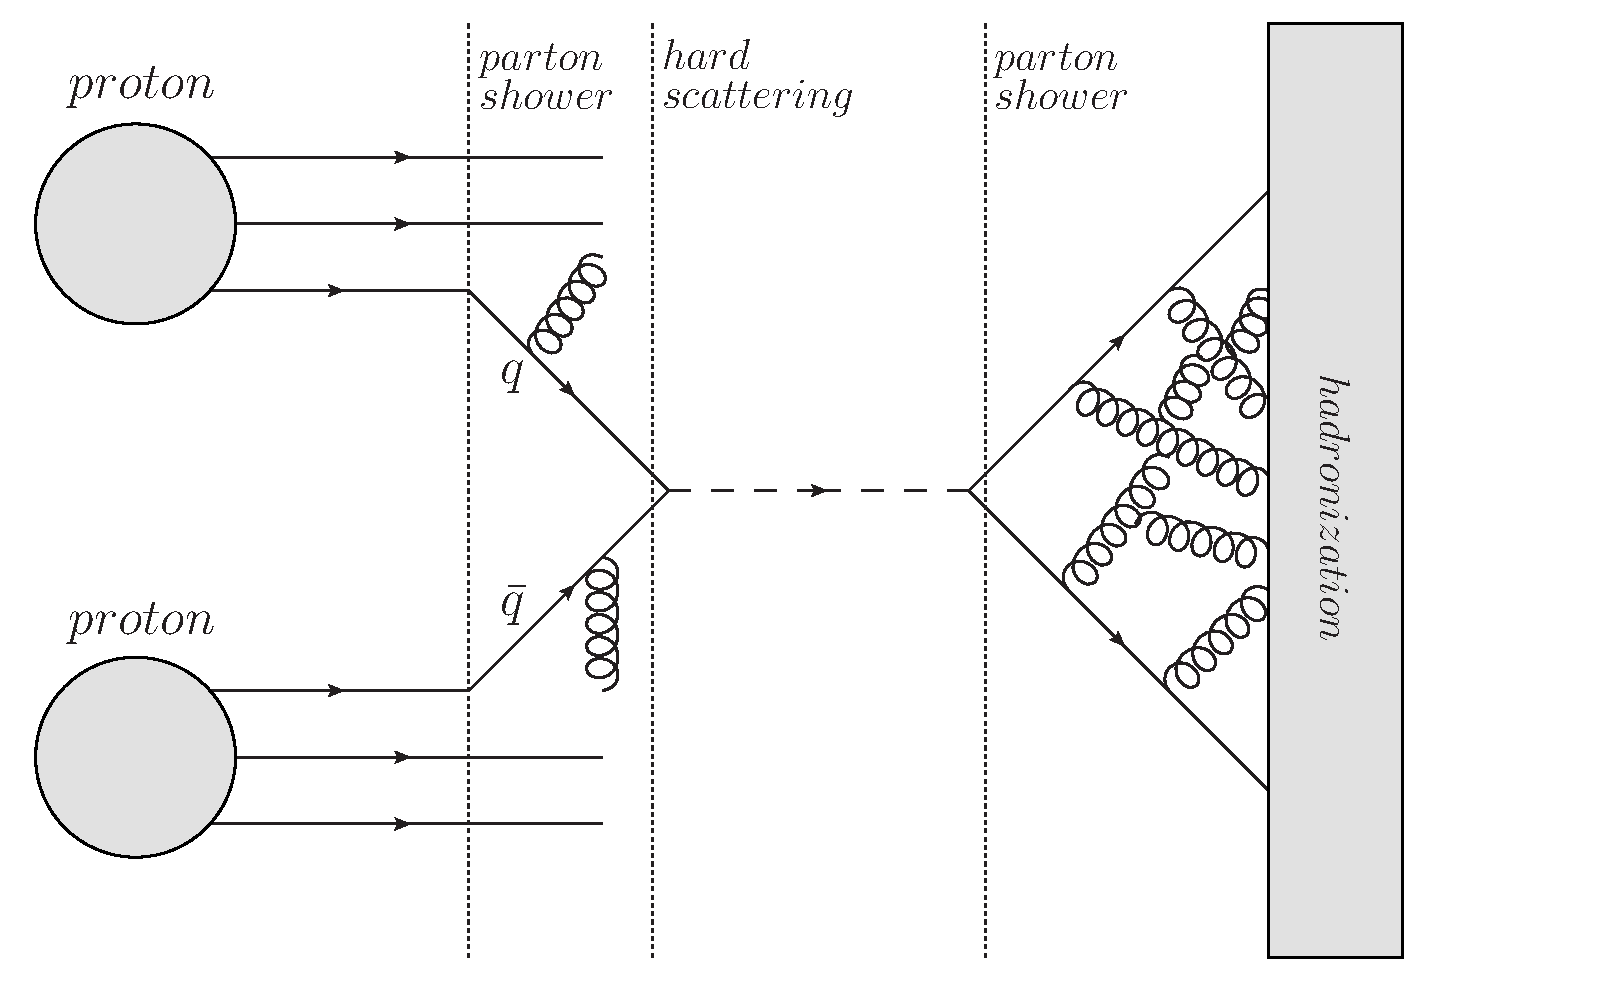
\includegraphics[width=0.8\textwidth]{figures/THEORY_qqbar.eps}
\caption{The deep inelastic scattering of two protons. The three main phases of the process are shown: initial radiation, the hard scattering itself, when the gauge boson is produced, and a final state radiation. If the gauge boson decayed into quarks, the hadronization process takes place in the end, when these quarks decay into color-neutral hadrons.}
\label{fig:THEORY_pp}}
\end{figure}

The process of the $pp$ collision is shown on Fig.~\ref{fig:THEORY_pp}. The three stages of the collision can be calculated by theory, with the use of the perturbative theory, but the difficulty of such calculations for the high orders of radiation processes makes it practically impossible. The three processes are calculated separately, with initial and final state radiations being calculated by the approach called the parton shower: the radiation process of each quark is calculated independently. The hard scattering itself can be calculated in leading order (LO, no radiative corrections), next to leading order (NLO, one radiative corrections), next to next to leading order (NNLO) and so on. Usually one radiative correction is used (NLO), which gives a result with an acceptable error, and is not difficult to calculate.

\begin{figure}
\center{
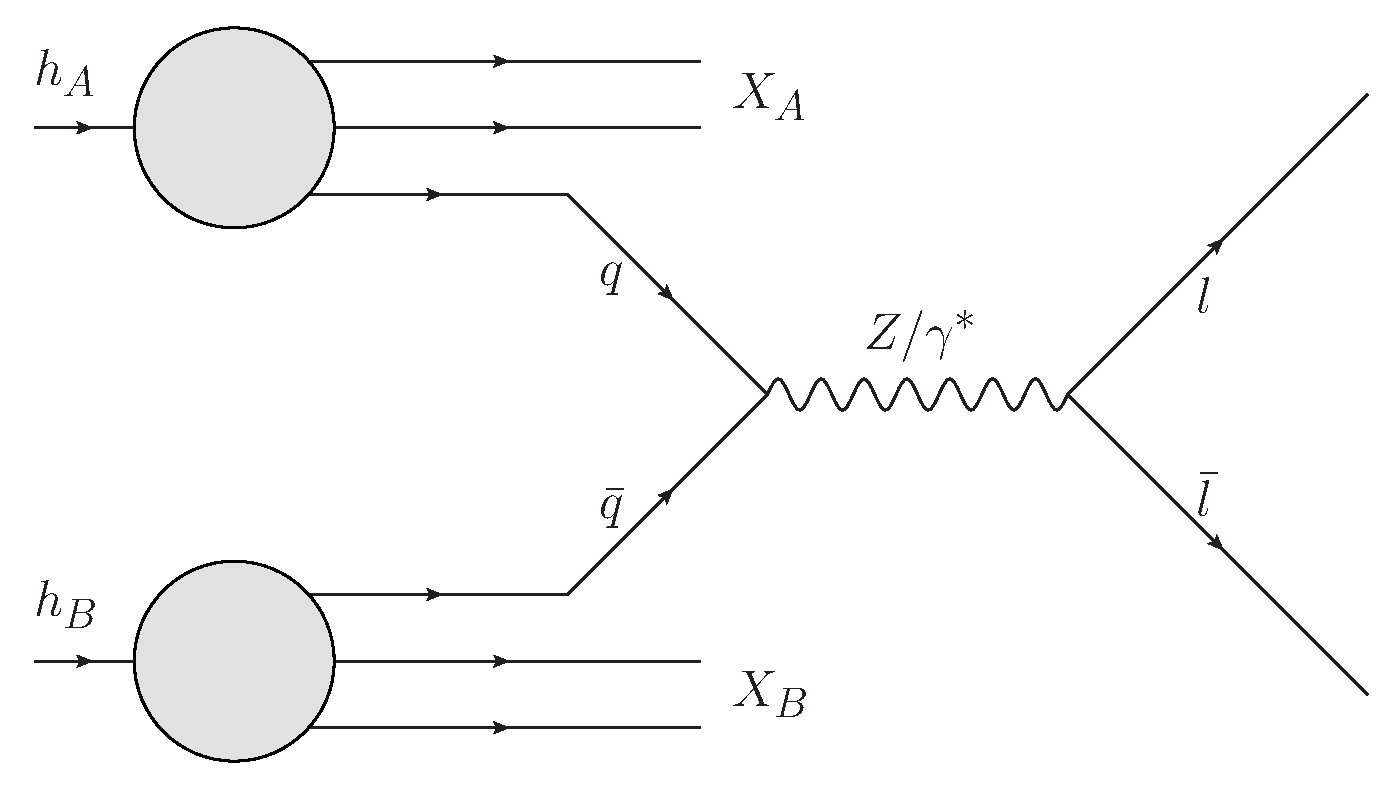
\includegraphics[width=0.8\textwidth]{figures/THEORY_DY.eps}
\caption{The Drell-Yan process in leading order. A quark from one hadron and an antiquark from another annihilate and produce a vector boson (photon or Z) which decays into lepton-antilepton pair. The remaining quarks of the initial hadrons do not interact between each other.}
\label{fig:THEORY_DY}}
\end{figure}

Z boson is produced during the Drell-Yan process, which is shown on Fig.~\ref{fig:THEORY_DY}. The process in leading order (also called the tree-level Drell-Yan) involves only a quark and an antiquark producing a boson which in turn decays into a lepton-antilepton pair.

To properly calculate a theoretical prediction for such a process, the PDFs must be applied to both interacting protons, which complicates the calculations and increases the resulting error. This is common problem of hadron colliders as opposed by lepton or $ep$ ones (while $ep$ colliders do use PDFs, they depend on it much less than the $pp$ ones). But because of it's high rest mass, hadrons can be accelerated to the much higher energies, which makes hadron colliders still preferable for certain tasks despite this shortcoming.

\section{Theoretical predictions for the \Zee\ cross-section}

There are several processes where the events can be clearly filtered from the background. The \Wenu\ and \Zee\ decays are the examples of such processes. The reason for this is because their decays have resonance in LHC, which outstands on the mass-spectrum from the others, like $J/\Psi$, $Y$, and di-boson decays. The electrons and the muons are the particles that undergo reconstruction and identification with best efficiencies, and the aforementioned decays have no hadronization phase which would result in jets, which have large resolution and scale errors. The cross-sections of such processes can thus be measured with high precision, and are important in different aspects.

While the \Zee\ analysis can be used for several things, including the researches on $\alpha_{s}$ constant and forward-backward asymmetry, the main application for the cross-section itself would be the PDF fits. The theoretical prediction for the Drell-Yan \Zgee\ process in LO is as follows~\cite{lib:theory_Z-c-s}:
\begin{equation}
\label{eq:theory_c-s}
\frac{d^{2}\sigma}{dM_{ee}dy} = \frac{4\pi\alpha^{2}_{s}(M_{ee})}{9}2M_{ee}\cdot P(M_{ee})\cdot\Phi(x_{1},x_{2},M^{2}_{ee})\,.
\end{equation}
Here the $M_{ee}$ is the mass of the boson, the $y$ is the boson rapidity, the $P(M)$ is the propagator term and the $\Phi(x_{1},x_{2},M^{2})$ the parton distribution function that depends on the $x$ parameter of both quark and antiquark. This cross-section is a sum of contribution from both $Z$ and $\gamma^*$ process as well as interference thereof. For the photon process the propagator and the PDF are given as

\begin{equation}
P_{\gamma}(M_{ee}) = \frac{1}{M^{4}_{ee}}\,,\,\;\Phi_{\gamma} = \sum_{q} e^{2}_{q} F_{\qqbar} \,.
\end{equation}

It can be seen that the propagator term $P_{\gamma}$ suppresses the photon contribution for the high-mass ($M_{ee} \gg M_{Z}$) and the mass peak ($M_{ee} \approx M_{Z}$) analyses.

For the $Z/\gamma$ interference contribution the same terms can be given as
\begin{equation}
\begin{gathered}
P_{Z\gamma}(M_{ee}) = \frac{k_{Z} \cdot v_{e} \cdot (M_{ee}^{2} - M_{Z}^{2})}{M_{ee}^{2} \cdot ((M_{ee}^{2} - M_{Z}^{2})^{2} + (\Gamma_{Z}M_{Z})^{2})}\,,\,\;
\Phi_{Z\gamma} = \sum_{q} 2e_{q}v_{q} F_{\qqbar} \,,\\
k_{Z} = \frac{1}{4\sin^{2}\theta\cos^{2}\theta} \,, \,\; \cos\theta = \frac{M_{W}}{M_{Z}} \,,
\end{gathered}
\end{equation}
Where $\theta$ is a $\theta_{W}$ - a weak mixing angle. The contribution of this component is proportional to the vector coupling of the electron $v_{e}$, which is close to zero, so the contribution is also negligible.

And finally for the \Zee\ process itself the terms are as follows:

\begin{equation}
P_{Z}(M_{ee}) = \frac{k^{2}_{Z} \cdot (v^{2}_{e} + a^{2}_{e})}{(M^{2}_{ee} - M^{2}_{Z})^{2} + (\Gamma_{Z}M_{Z})^{2}}\,,\,\;
\Phi_{Z} = \sum_{q} (v^{2}_{q} + a^{2}_{q}) F_{\qqbar} \,.
\end{equation}

As it is seen from this, the PDFs are included in the cross-section formula as a direct factor, so the double-differential cross section can be directly used to conduct the PDF fits.

\begin{figure}
\center{
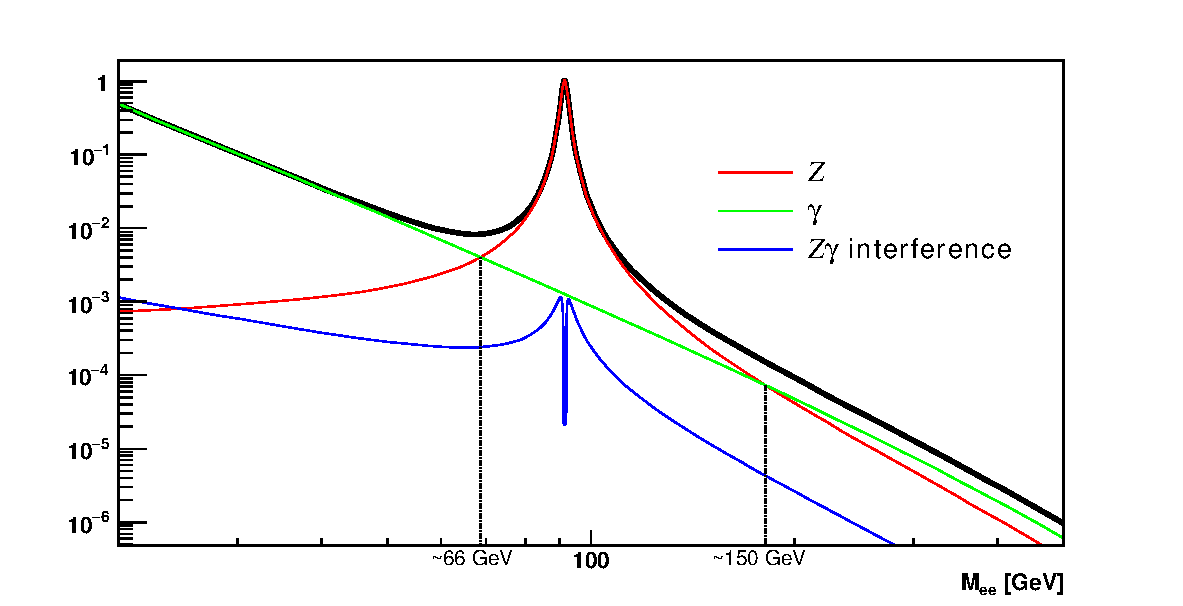
\includegraphics[width=0.8\textwidth]{figures/THEORY_Zcs.pdf}
\caption{The theoretical predictions for the cross-sections of the Drell-Yan \Zgee\ processes, normalized to \Zee\ peak value. The cross-sections were calculated in leading order, using the CT10 PDF set.}
\label{fig:THEORY_Zcs}}
\end{figure}

All the cross-sections can be seen together on Fig.~\ref{fig:THEORY_Zcs}. The cross-section for \Zee\ process is higher then that of \gee\ only around the peak region, starting from $\sim$66~GeV up to $\sim$150~GeV. The region is divided into two: the peak region ($66 - 116$~GeV) and the high mass region ($116 - 150$~GeV). The boundary between the regions is picked in such a way that the Z boson mass was at the center of the peak region.


\begin{figure}
\center{
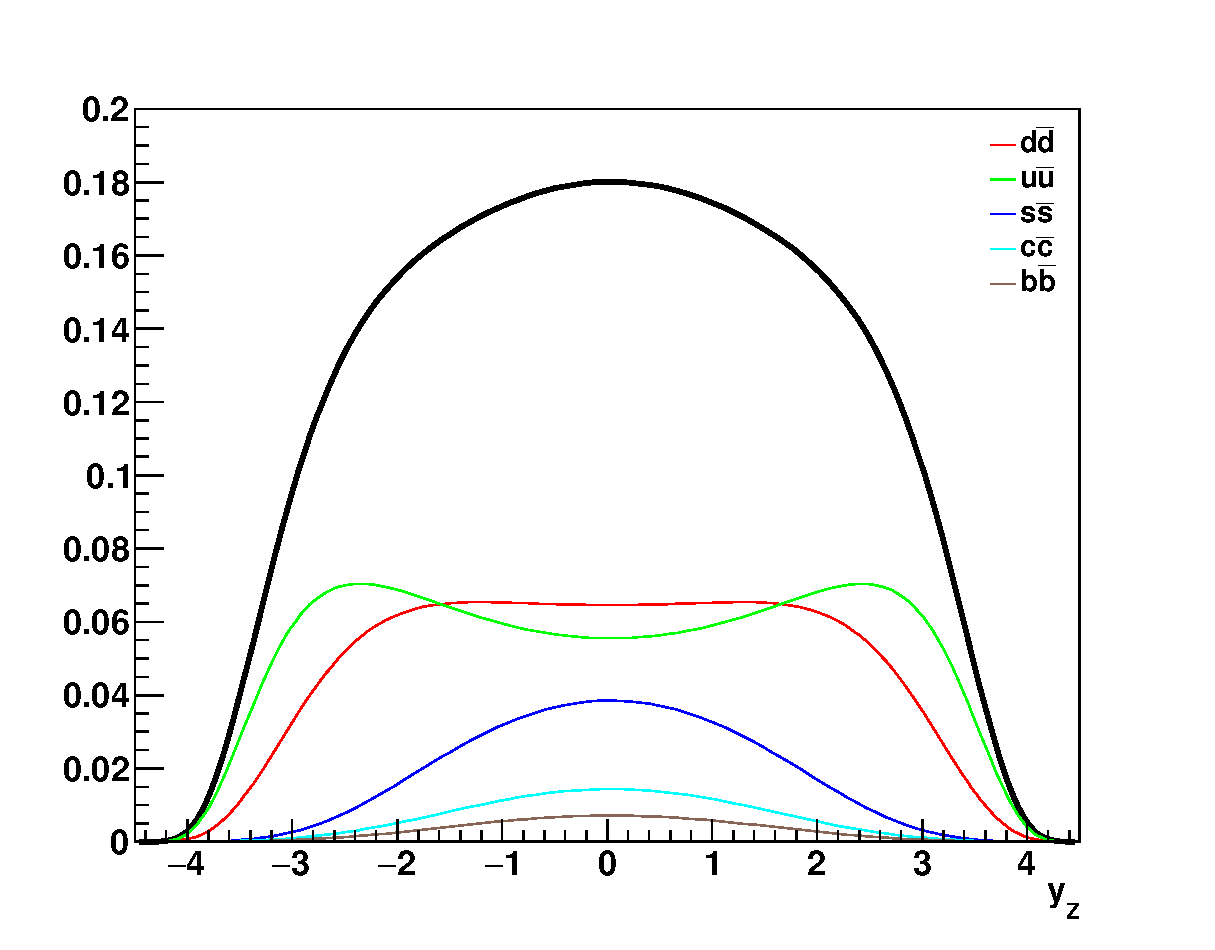
\includegraphics[width=0.48\textwidth]{figures/THEORY_ZeePDF.eps}
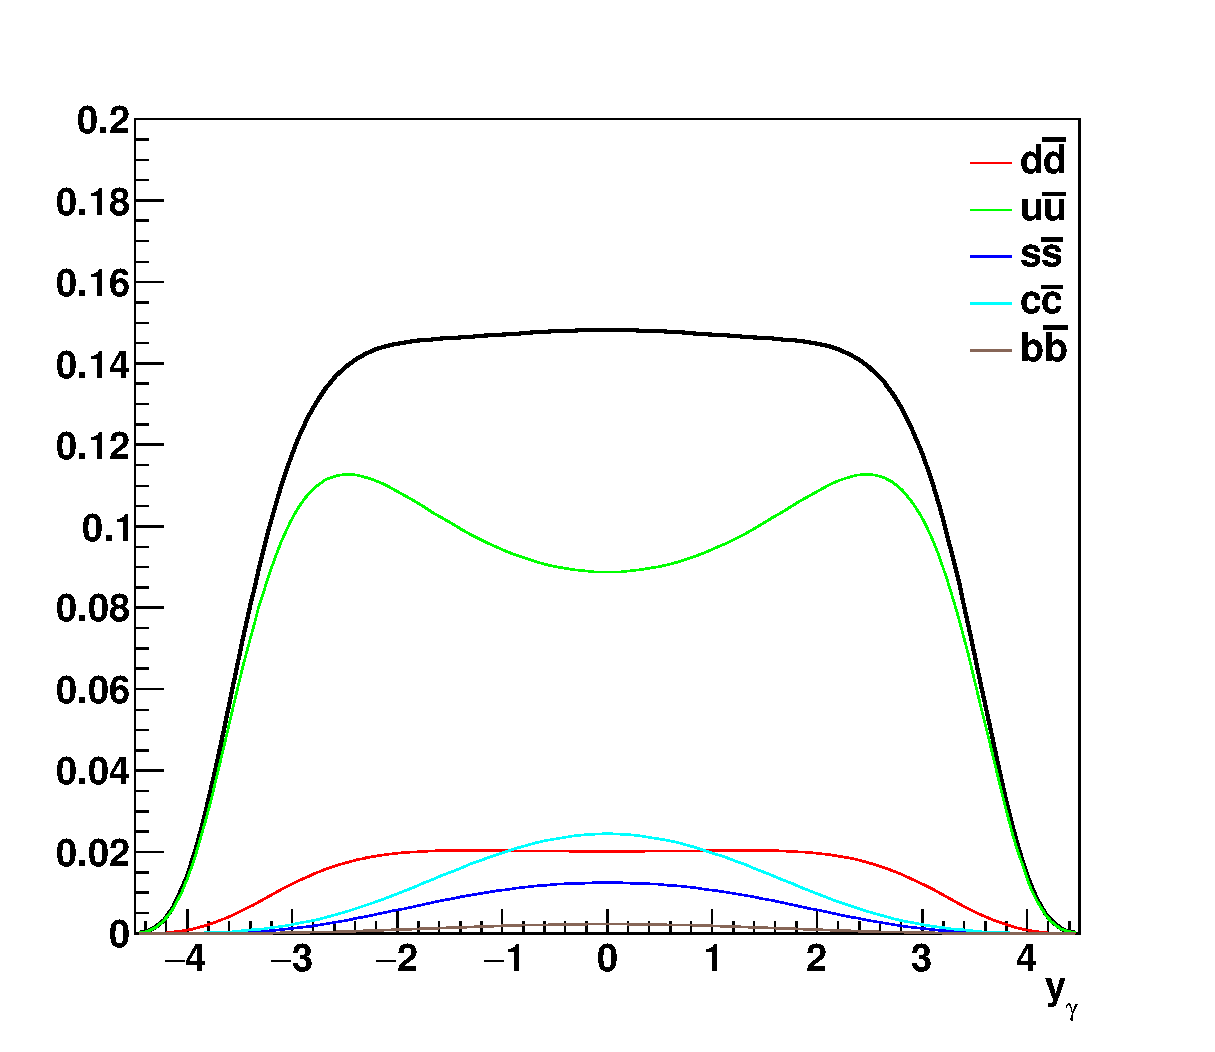
\includegraphics[width=0.48\textwidth]{figures/THEORY_GeePDF.eps}
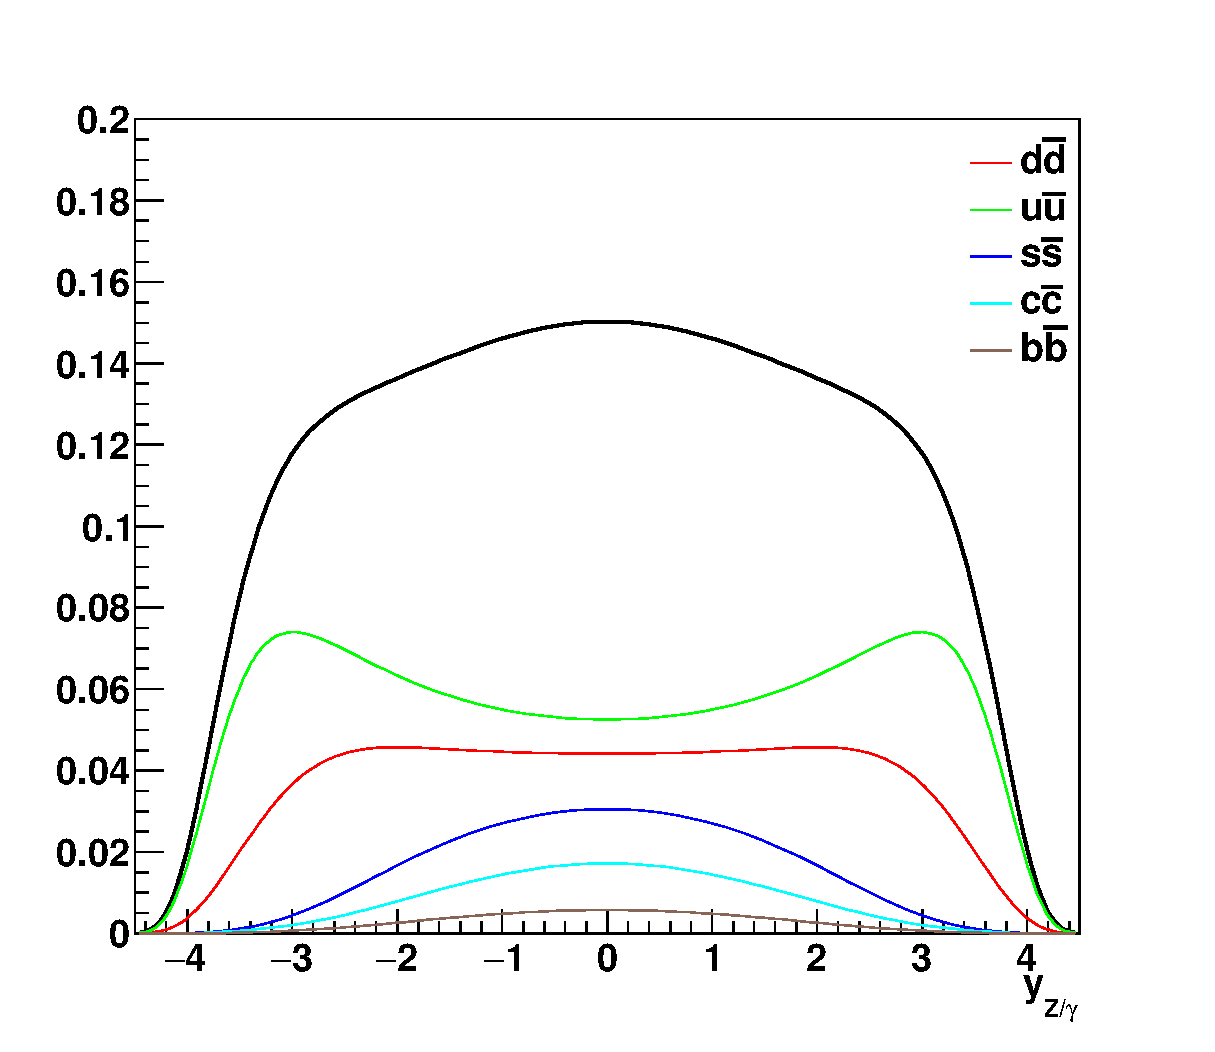
\includegraphics[width=0.48\textwidth]{figures/THEORY_ZGeePDF.eps}
\caption{The PDF decomposition of the normalized cross-sections of the Drell-Yan processes. The decomposition of the \Zee\ (left), \gee\ (right) and $Z/\gamma$ interference (bottom) processes are shown. The cross-sections were calculated in leading order, using CT10 PDF set}
\label{fig:THEORY_PDF}}
\end{figure}

The PDF decomposition for the two dominant processes is shown on Fig.~\ref{fig:THEORY_PDF}. There, the contribution from the various quarks to the final cross section is shown. It can be seen that \Zee\ central-central cross-section is dominated by \antibar{d} interactions, while in case of the central-forward the \antibar{u} is larger. For the \gee\ cross-section the \antibar{u} interactions are by far the largest contributors.
